\chapter{Efeito da ureia}
	\section{Motivação}
	A ureia demonstrou um comportamento que divergiu bastante dos outros aditivos. Por esse motivo, ela será estudada um pouco mais profundamente. Porém, a ação do salicilato de sódio não receberá muito enfoque, para simplificar o sistema. Portanto, foi estudado principalmente o efeito da ureia em soluções de CTAB, TTAB e DTAB, com concentrações diferentes de ureia e de surfactante.
	
	Ocorre a formação de um precipitado esbranquiçado em soluções de surfactante em concentrações maiores que 35\% de ureia. Isso ocorre a temperatura ambiente. Quando a solução é aquecida acima de cerca de 35ºC, ela se torna transparente. Esse comportamento foi estudado, variando-se o surfactante, sua concentração, e a concentração de ureia. Desses sistemas, foram estudadas as características térmicas, a estrutura da mesofase, e a reologia da fase esbranquiçada.
	
	\section{Calorimetria diferencial de varredura (DSC)}

		Foram preparadas soluções de ureia, em várias concentrações, com três surfactantes (CTAB, TTAB e DTAB), em três concentrações. Os termogramas resultantes foram organizados em figuras de modo a facilitar comparações. A tabela \ref{tab:refs_DSC} lista as comparações realizadas e em quais figuras estão.
        
        \begin{table}[H]
            \IBGEtab{%
                \caption{Comparações de termogramas de amostras de surfactante (concentração em \mM)e ureia (\% m/m), e suas respectivas figuras}
                \label{tab:refs_DSC}
                }%
                {%
                \begin{tabular}{l c c}
                    \toprule
        			%\centering
        			Surf. \mM     & \% Ureia		& Figura 			\\
        			\midrule
        			CTAB 100	  & 38--45			& \ref{fig:DSC_CTAB_UR38-45}	\\
        			CTAB 100, 200, 300	& 45, 40	& \ref{fig:DSC_CTAB_UR40-45}	\\
        			TTAB 100, 200, 300	& 45, 40	& \ref{fig:DSC_TTAB_UR_40-45}	\\
        			DTAB 100, 200, 300	& 45, 40	& \ref{fig:DSC_DTAB_UR_40-45}	\\
        			CTAB, TTAB, DTAB 100	& 45	& \ref{fig:DSC_Surf_100mm_45p}	\\
        			CTAB, TTAB, DTAB 200	& 45	& \ref{fig:DSC_Surf_200mm_45p}	\\
        			CTAB, TTAB, DTAB 300	& 45	& \ref{fig:DSC_Surf_300mm_45p}	\\
        			\midrule
        			CTAB 100 NaSal 60	& 35, 40, 45	& \ref{fig:DSC_NaSal60}		\\
        			CTAB 100 NaSal 100	& 35, 40, 45	& \ref{fig:DSC_NaSal100}	\\
        			CTAB 100 NaSal 250	& 35, 40, 45	& \ref{fig:DSC_NaSal250}	\\
        			CTAB 100 NaSal 60, 100, 250 & 35 	& \ref{fig:DSC_NaSal_Ur35}  \\
        			CTAB 100 NaSal 60, 100, 250 & 40	& \ref{fig:DSC_NaSal_Ur40}  \\
        			CTAB 100 NaSal 60, 100, 250	& 45	& \ref{fig:DSC_NaSal_Ur45}  \\
        			\bottomrule
                \end{tabular}%
                }{}
        \end{table}
		
		% todo: cortar o número de figuras para diminuir repetição, adicionar outros gráficos mostrando como os parâmetros são afetados
		% todo: tirar CTAB 400 mM? Ele foje em muitos casos do esperado. Como explicar?
		
		\begin{figure}[H]
			\centering
			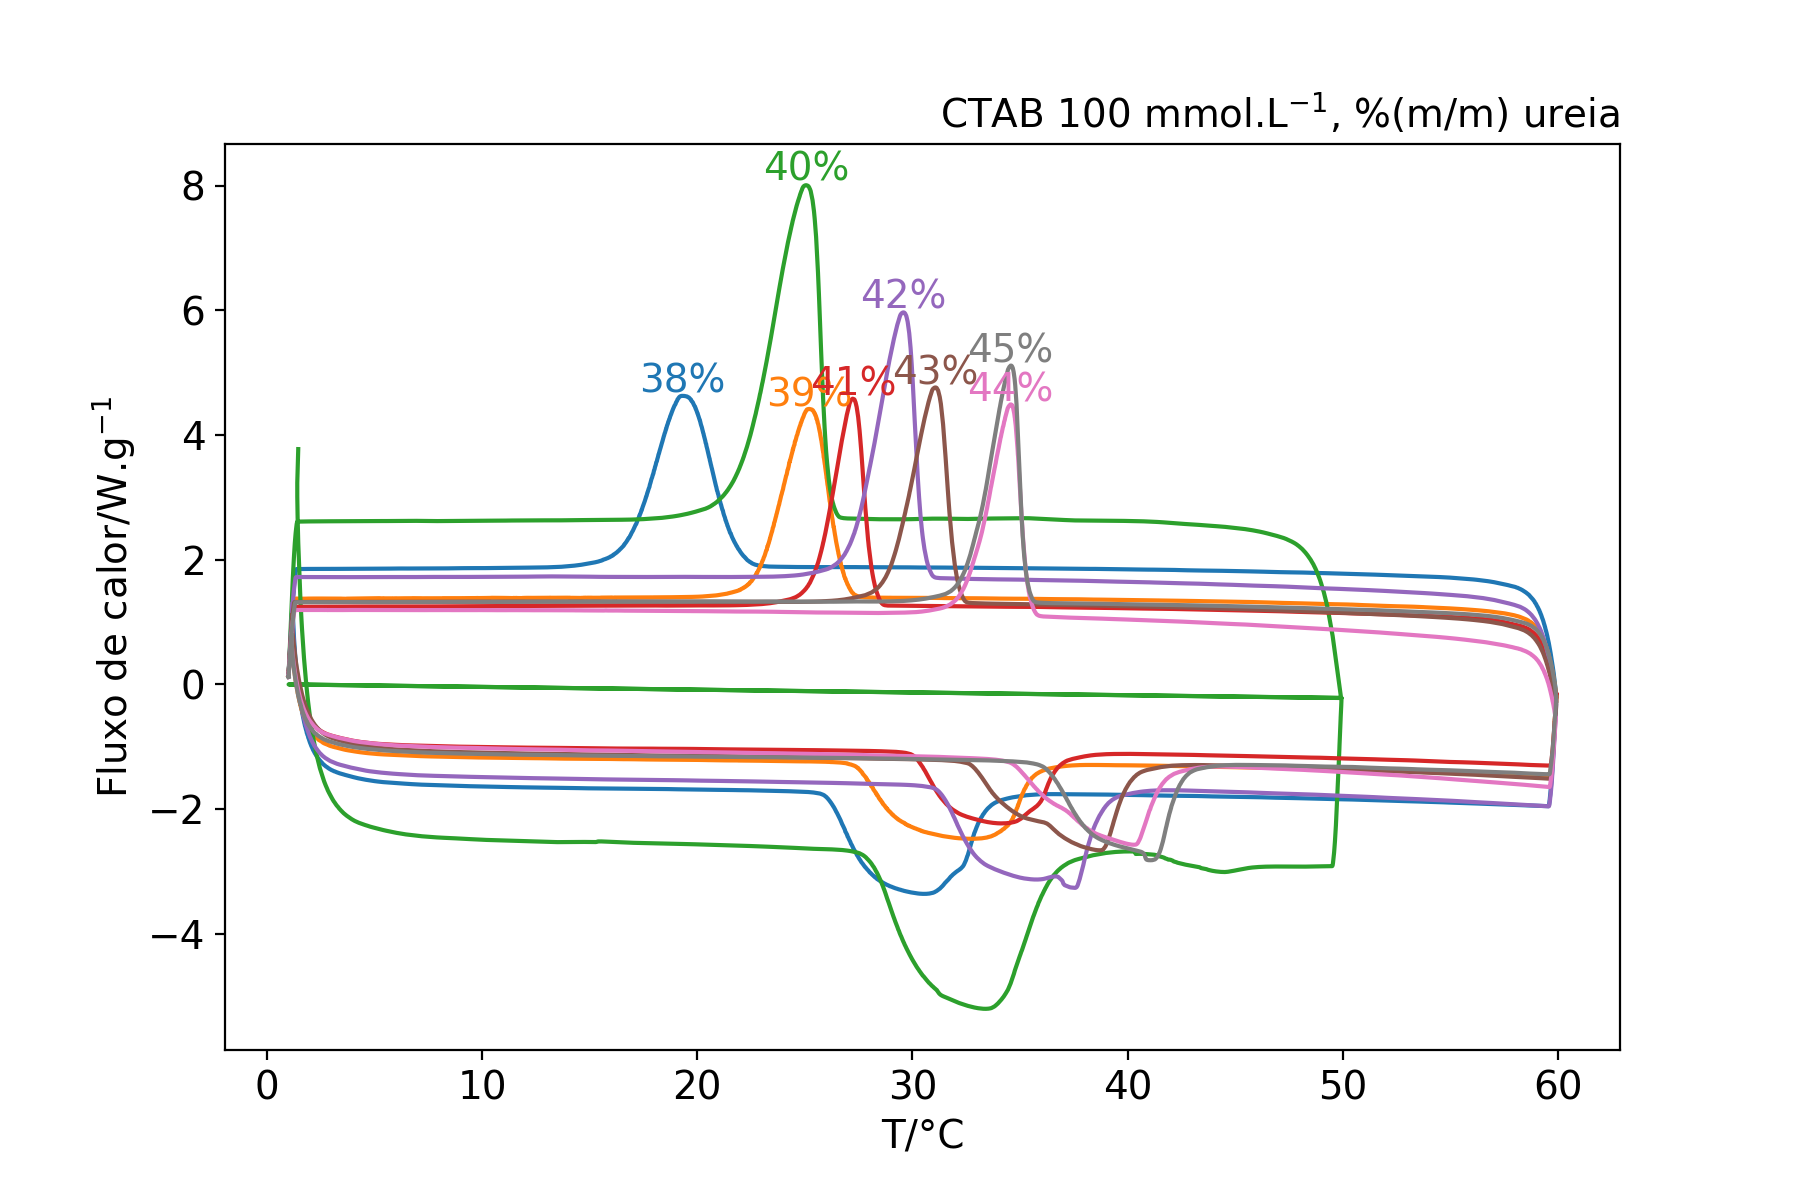
\includegraphics[width=0.75\textwidth]{./imagens/dsc/CTAB_porc_ur}
			\caption{Termogramas de soluções de CTAB 100 \mM{} em concentrações crescentes de ureia, de 38\% m/m a 45\% m/m}
			\label{fig:DSC_CTAB_UR38-45}
		\end{figure}
		
		\begin{figure}[H]
			\begin{subfigure}[t]{0.45\textwidth}
				\centering
				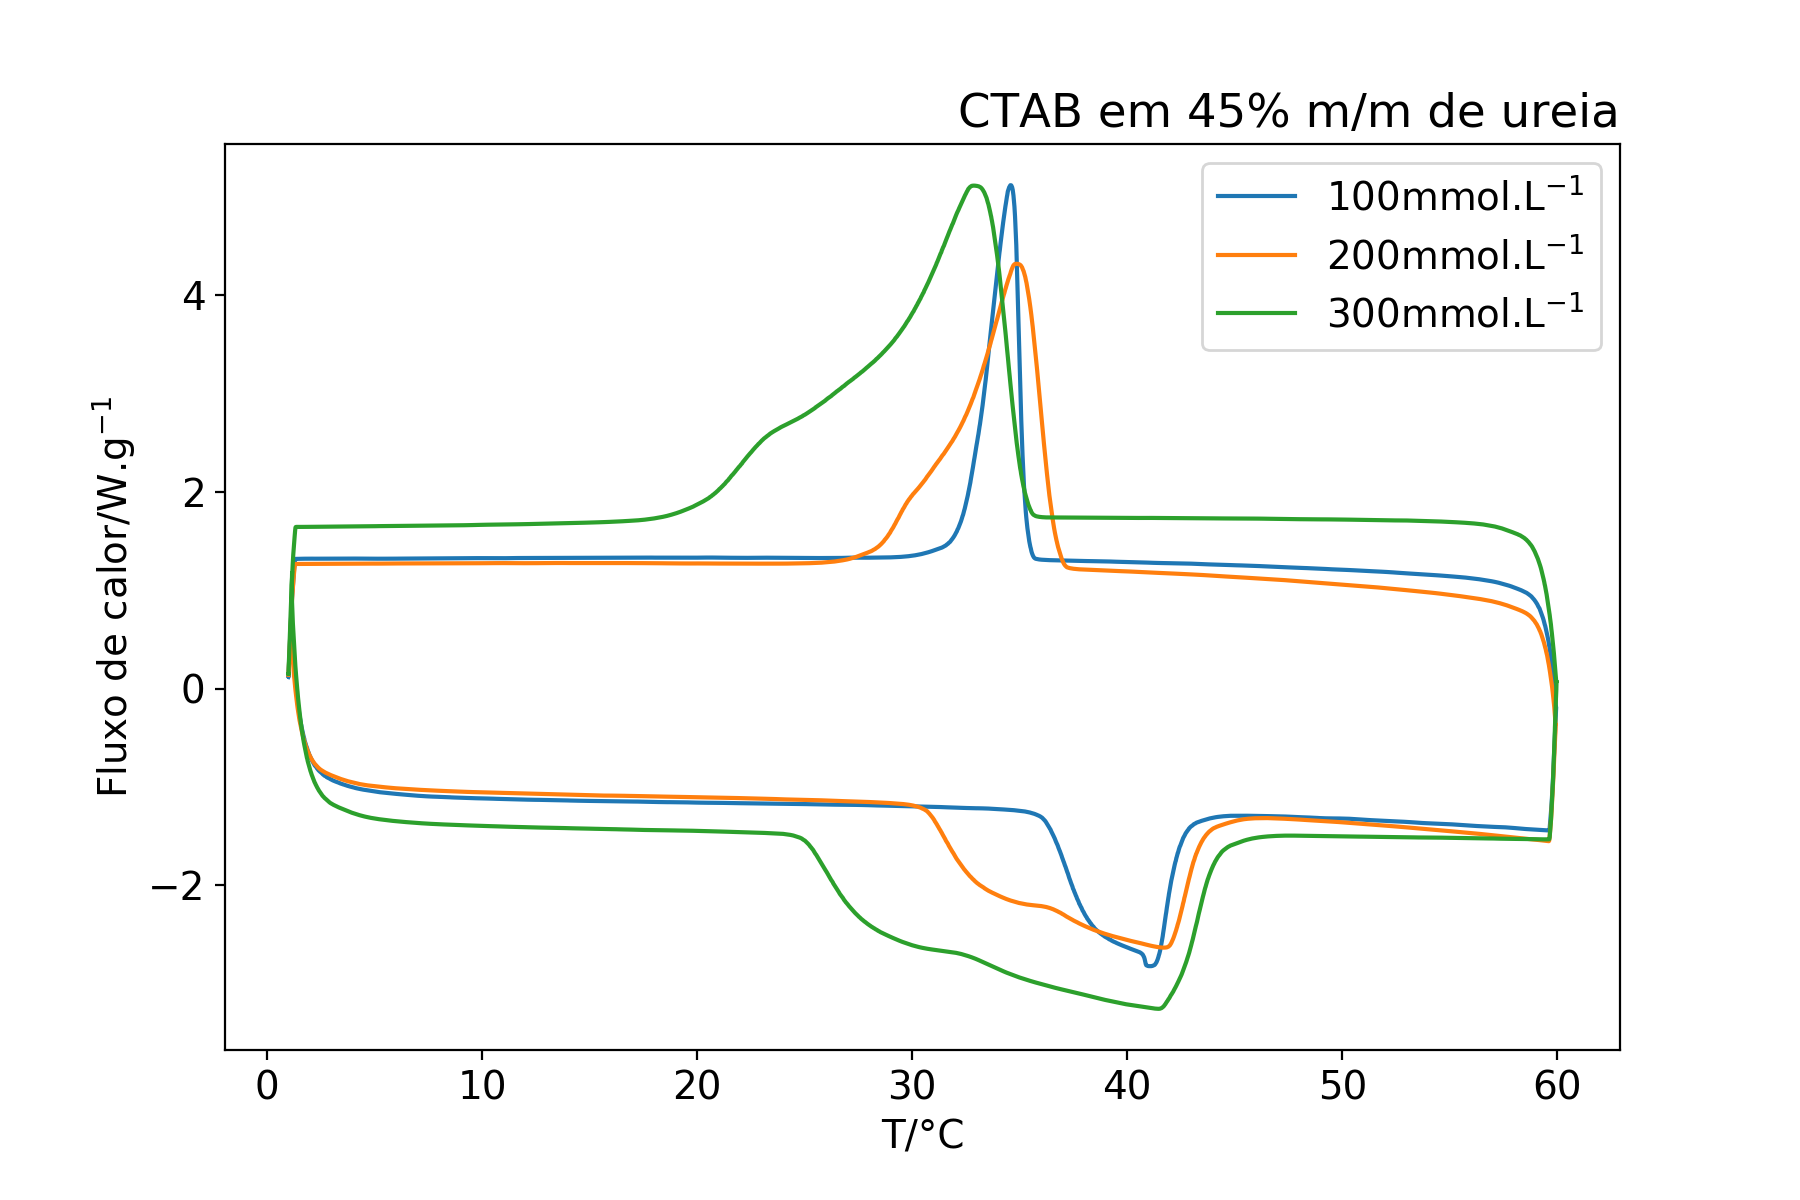
\includegraphics[width=\textwidth]{./imagens/dsc/CTAB_45p}
				\caption{45\% de ureia}
				\label{fig:DSC_CTAB_UR45}
			\end{subfigure} \qquad %
			\begin{subfigure}[t]{0.45\textwidth}
				\centering
				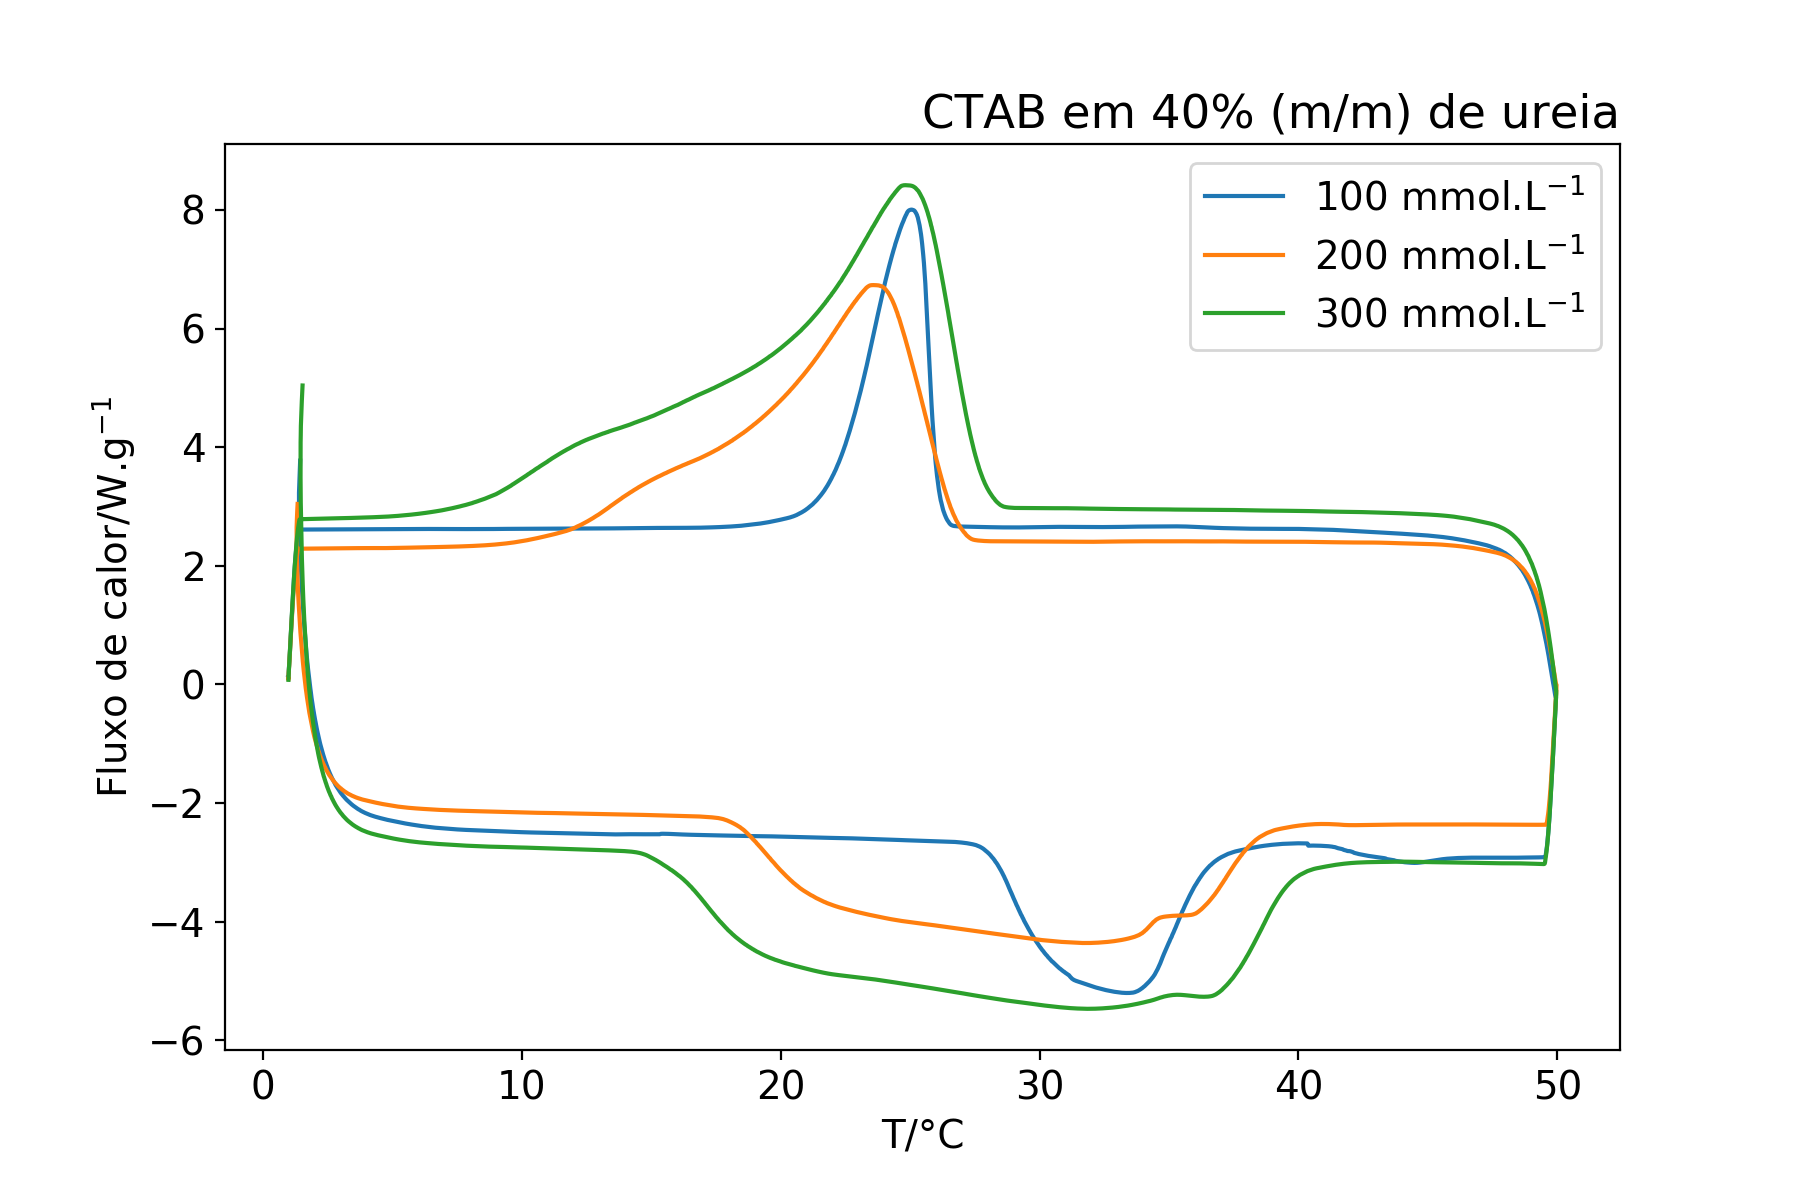
\includegraphics[width=\textwidth]{./imagens/dsc/CTAB_40p}
				\caption{40\% de ureia}
				\label{fig:DSC_CTAB_UR40}
			\end{subfigure}
			\caption{Termogramas de CTAB 100, 200 e 300 \mM{} em soluções em 45\% (\ref{fig:DSC_CTAB_UR45}) e 40\% (\ref{fig:DSC_CTAB_UR40})}
			\label{fig:DSC_CTAB_UR40-45}
		\end{figure}
	
		\begin{figure}[H]
			\centering
			\begin{subfigure}[t]{0.45\textwidth}
				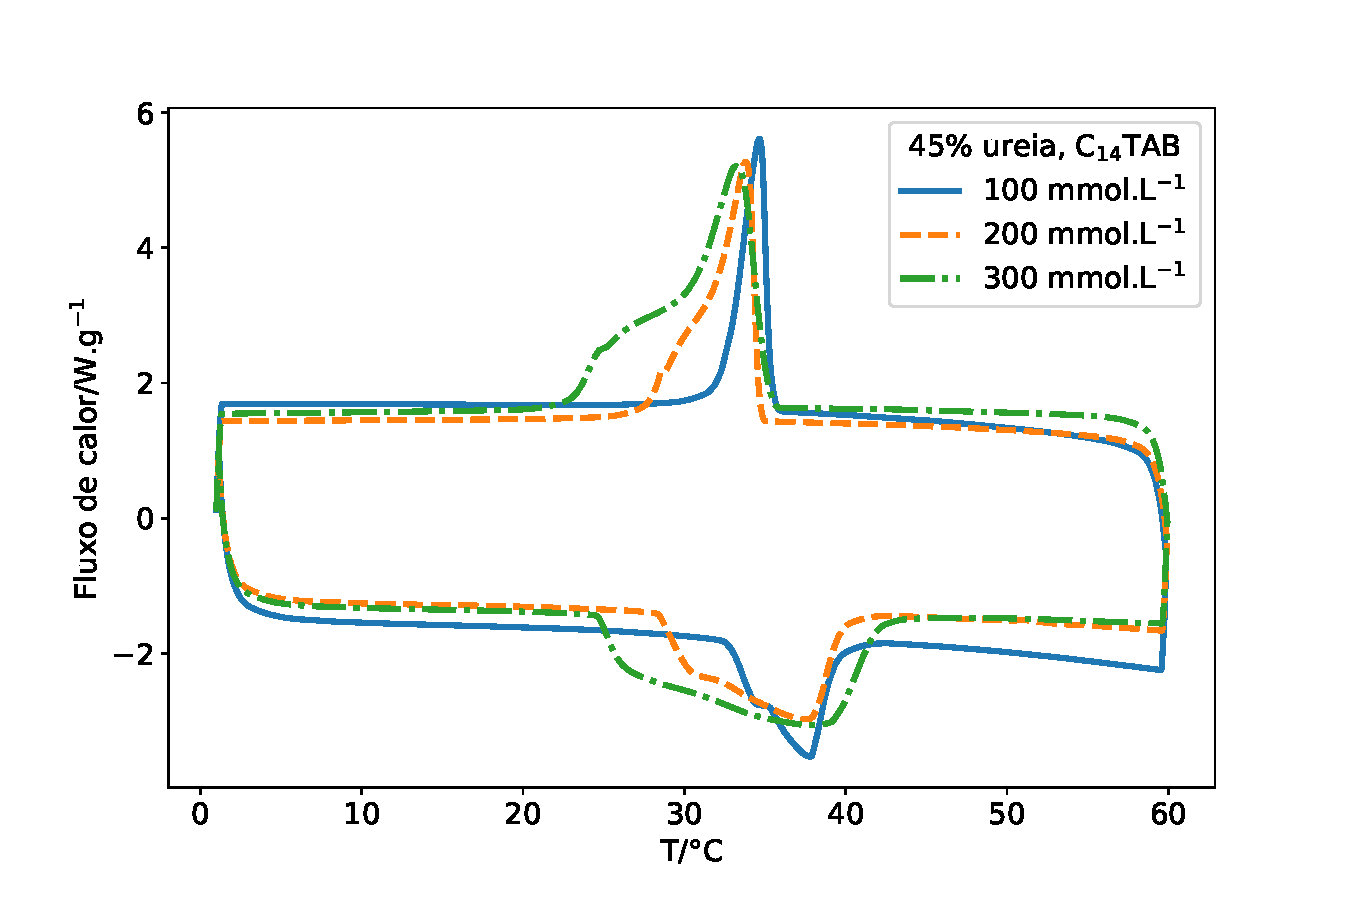
\includegraphics[width=\textwidth]{./imagens/dsc/TTAB_45p}
				\caption{45\% de ureia}
				\label{fig:DSC_TTAB_UR45}
			\end{subfigure} \qquad %
			\begin{subfigure}[t]{0.45\textwidth}
				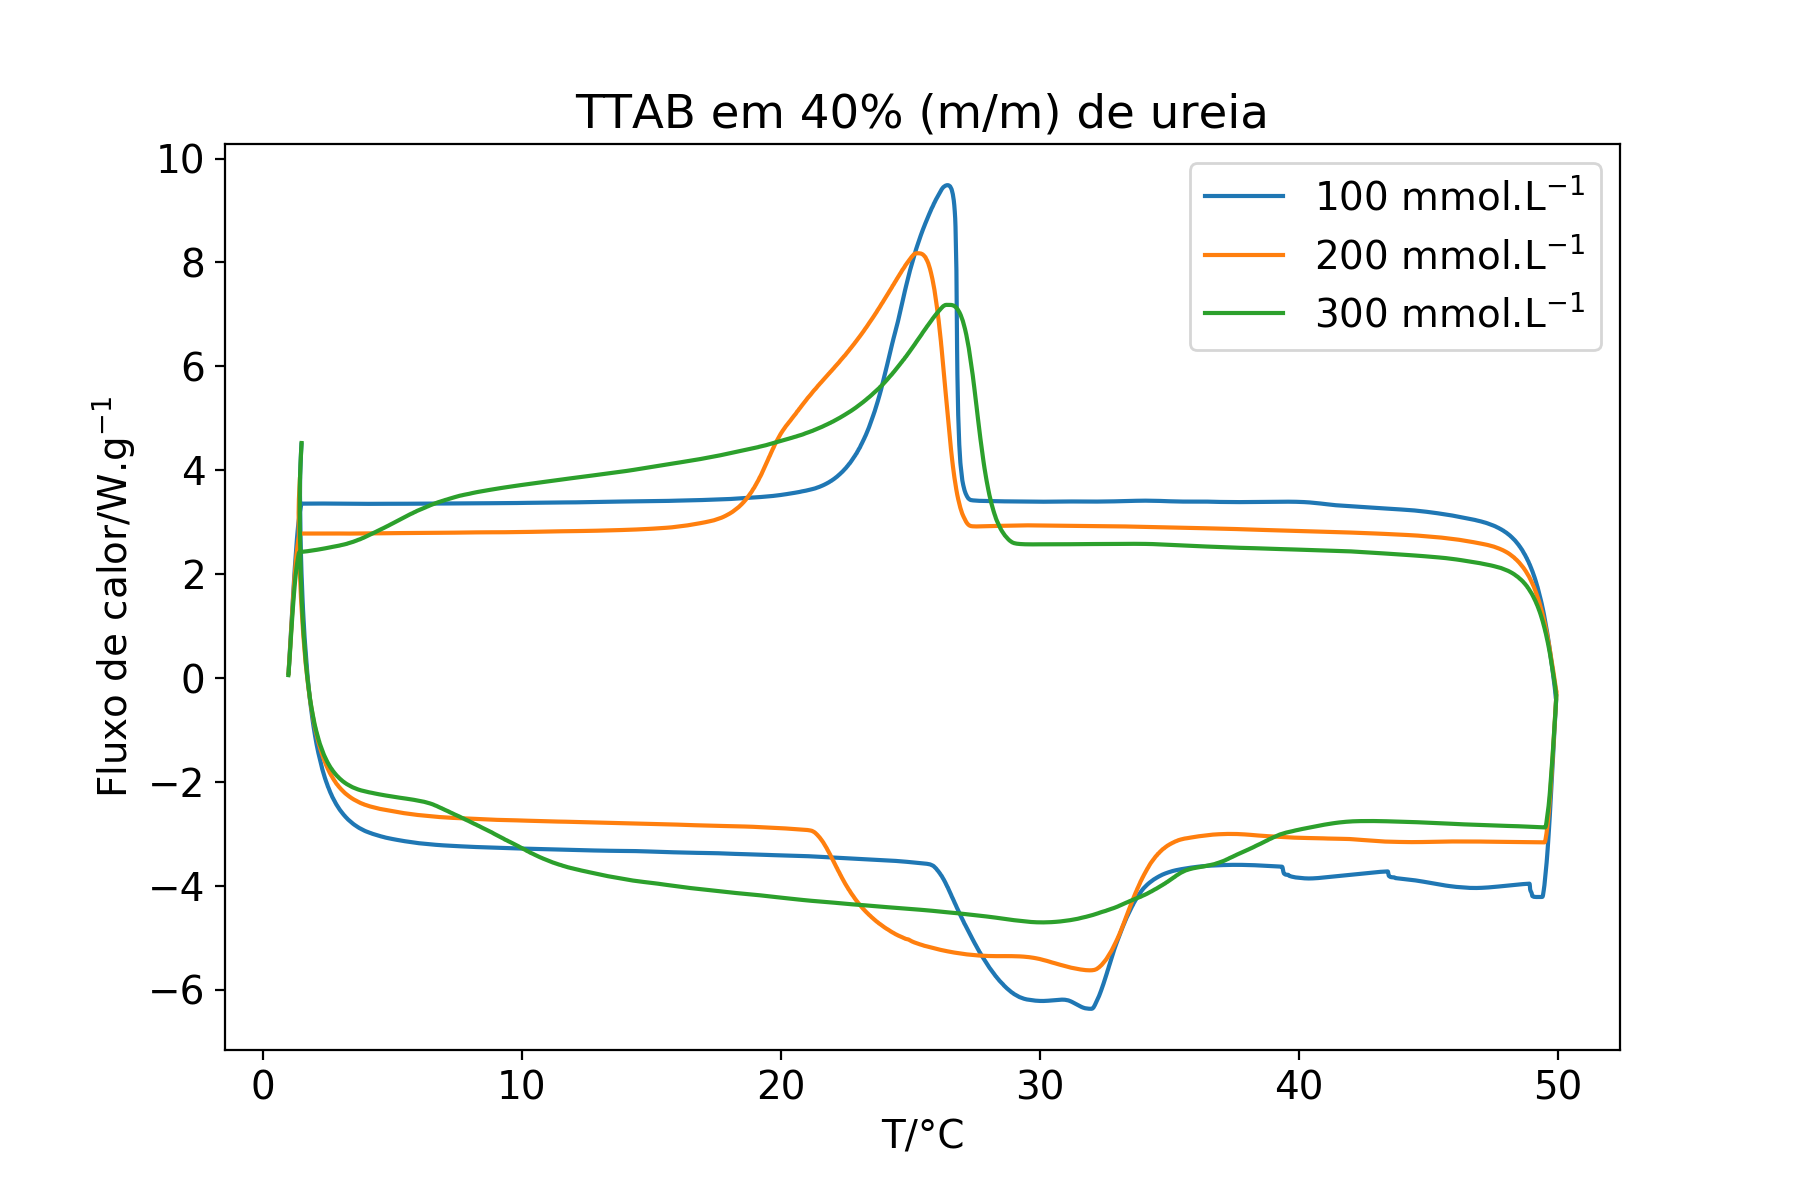
\includegraphics[width=\textwidth]{./imagens/dsc/TTAB_40p}
				\caption{40\% de ureia}
				\label{fig:DSC_TTAB_UR40}
			\end{subfigure}
			\caption{Termogramas de soluções de TTAB 100, 200 e 300 \mM{}, em 45\% (\ref{fig:DSC_TTAB_UR45}) e 40\% (\ref{fig:DSC_TTAB_UR40}) de ureia}
			\label{fig:DSC_TTAB_UR_40-45}
		\end{figure}
		
		\begin{figure}[H]
			\centering
			\begin{subfigure}[t]{0.45\textwidth}
				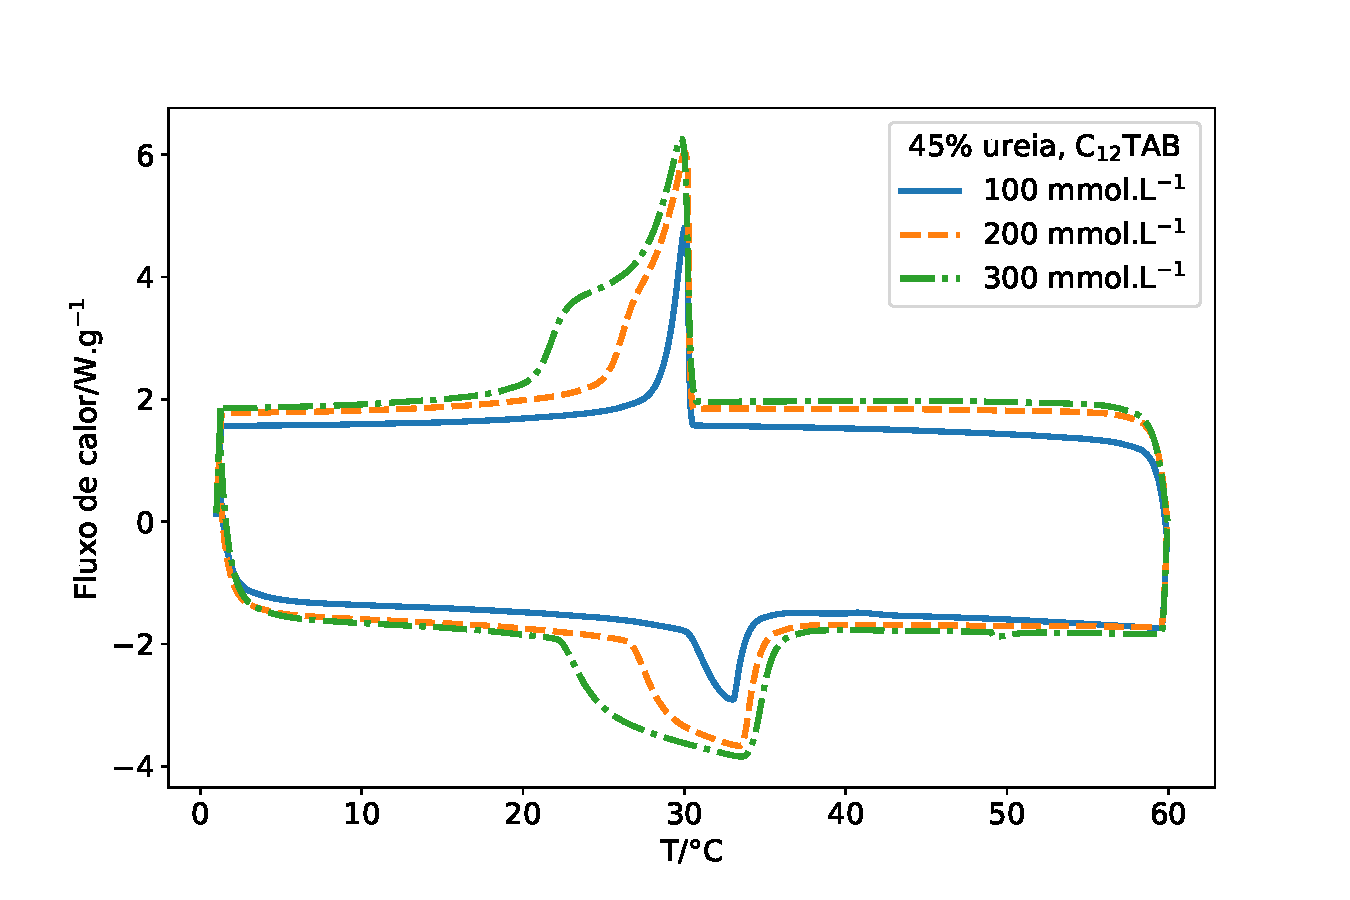
\includegraphics[width=\textwidth]{./imagens/dsc/DTAB_45p}
				\caption{45\% de ureia}
				\label{fig:DSC_DTAB_UR45}
			\end{subfigure} \qquad %
			\begin{subfigure}[t]{0.45\textwidth}
				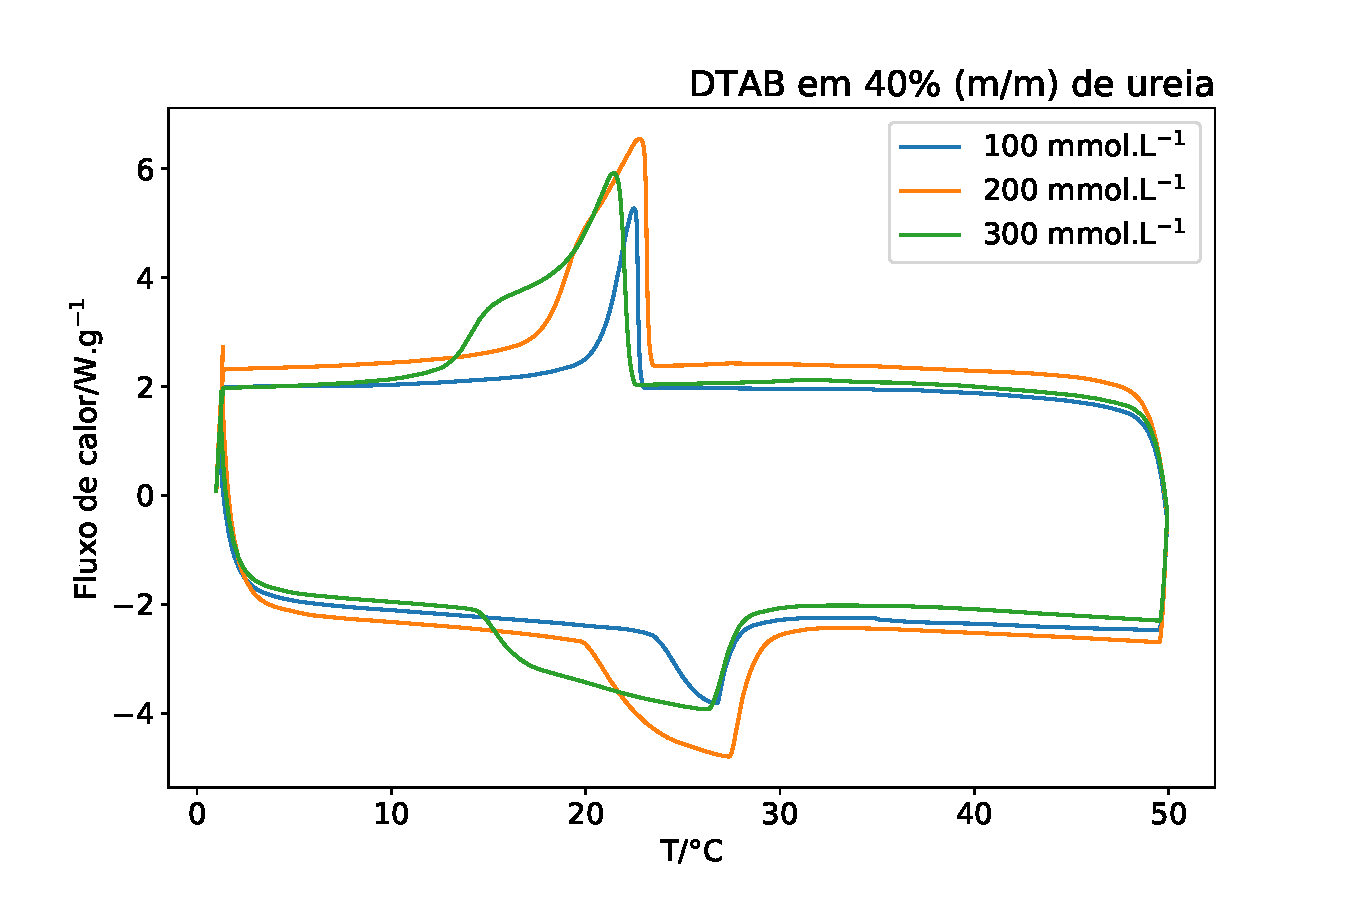
\includegraphics[width=\textwidth]{./imagens/dsc/DTAB_40p}
				\caption{40\% de ureia}
				\label{fig:DSC_DTAB_UR40}
			\end{subfigure}
			\caption{Termogramas de soluções de DTAB 100, 200 e 300 \mM{}, em 45\% (\ref{fig:DSC_DTAB_UR45}) e 40\% (\ref{fig:DSC_DTAB_UR40}) de ureia}
			\label{fig:DSC_DTAB_UR_40-45}
		\end{figure}
		
		
		% todo: verificar se a notação (C|T|D) é boa
		\begin{figure}[H]
			\centering
			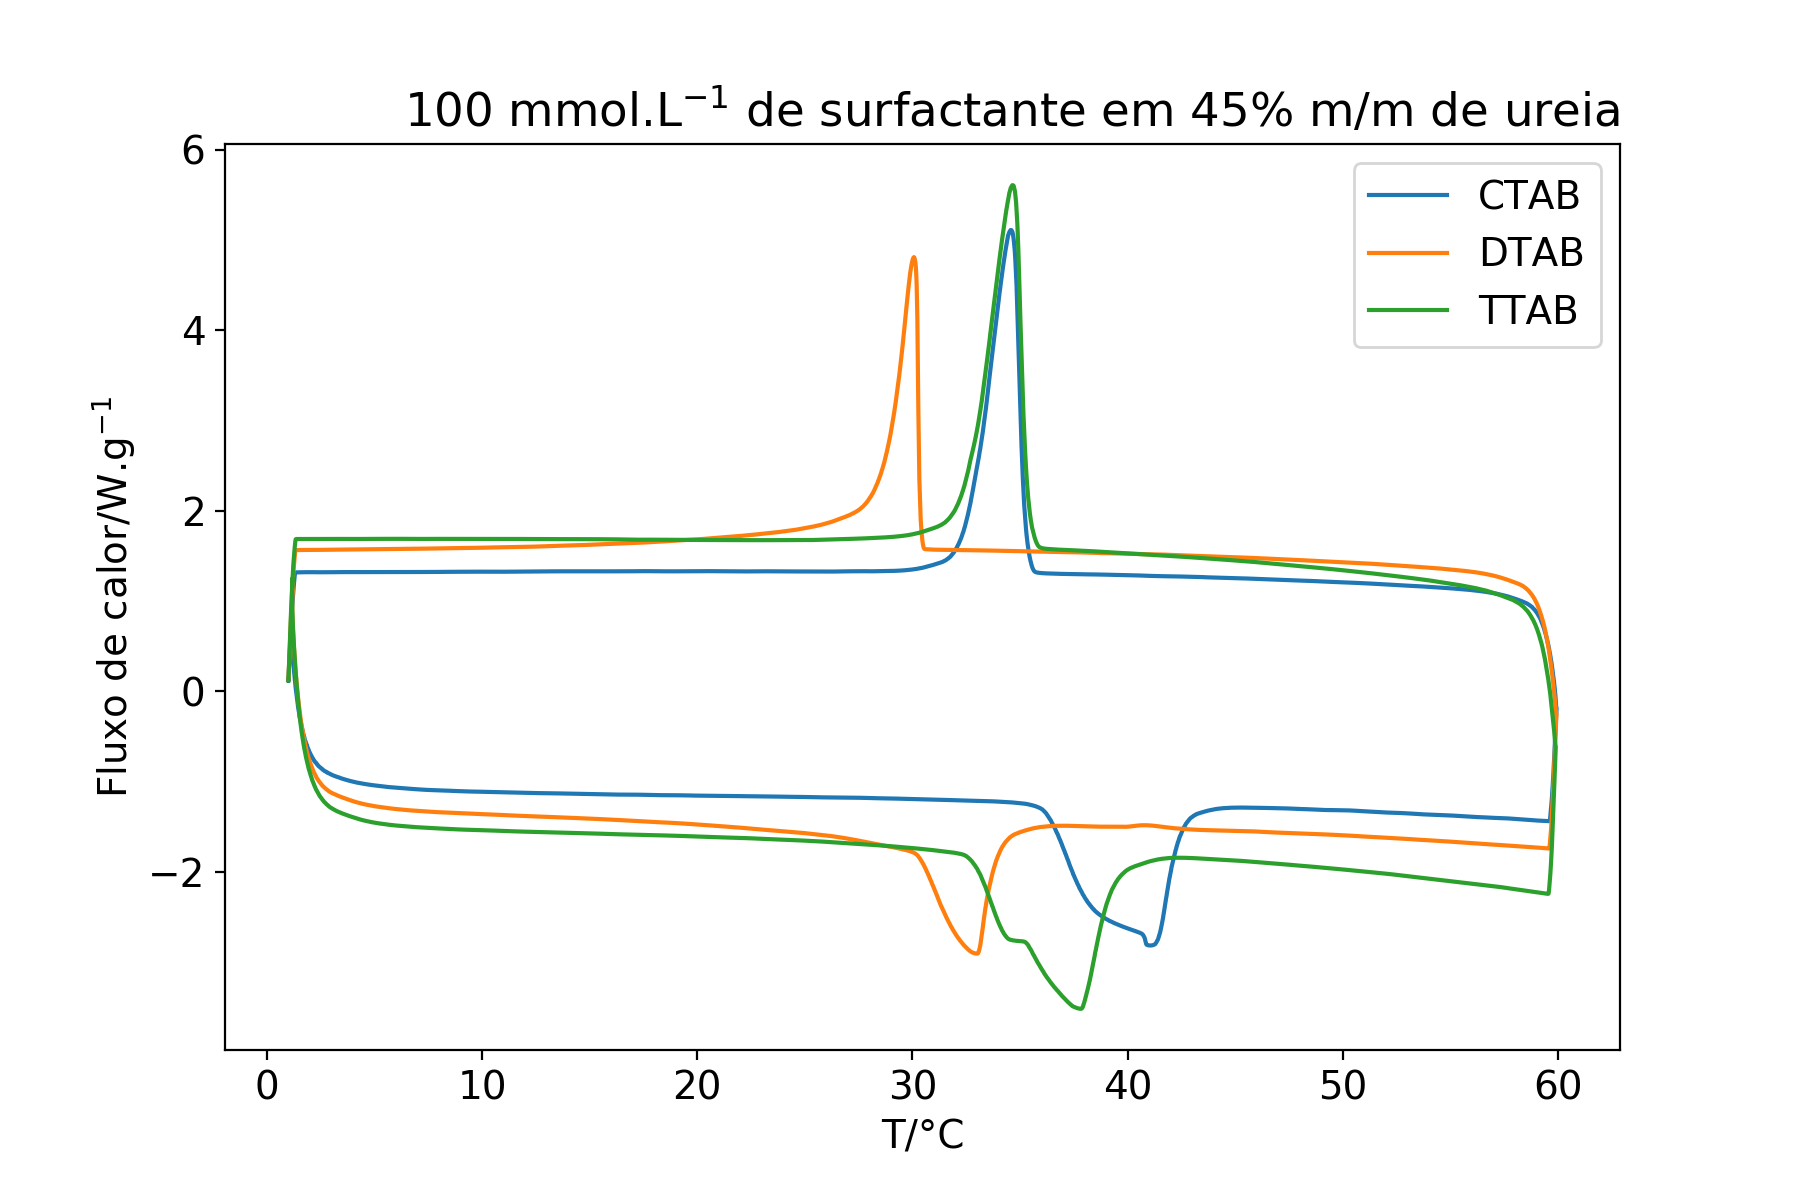
\includegraphics[width=0.60\textwidth]{./imagens/dsc/Surf_100mm_45p}
			\caption{Termogramas de soluções de (C|T|D)TAB 100 \mM{}, em 45\% de ureia}
			\label{fig:DSC_Surf_100mm_45p}
		\end{figure}
	
		\begin{figure}[H]
			\centering
			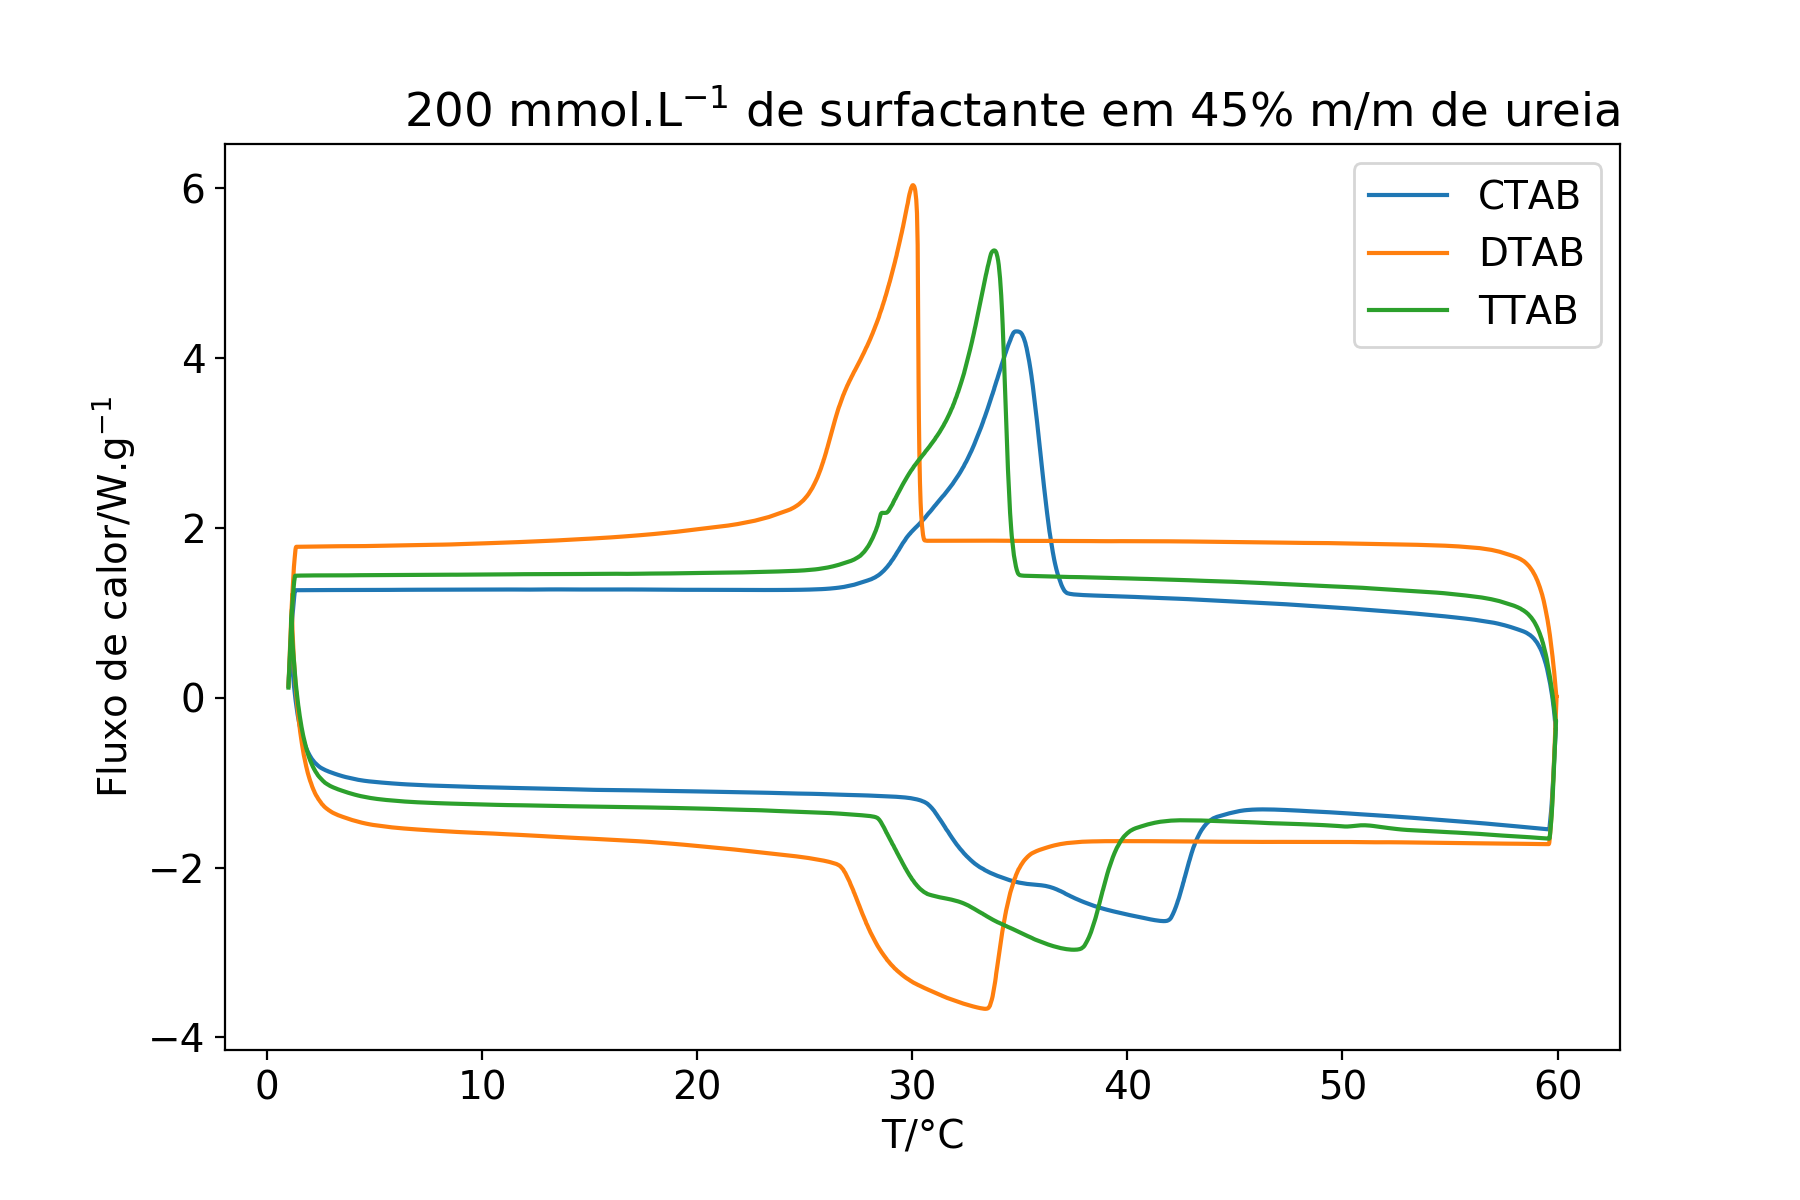
\includegraphics[width=0.60\textwidth]{./imagens/dsc/Surf_200mm_45p}
			\caption{Termogramas de soluções de (C|T|D)TAB 200 \mM{}, em 45\% de ureia}
			\label{fig:DSC_Surf_200mm_45p}
		\end{figure}
	
		\begin{figure}[H]
			\centering
			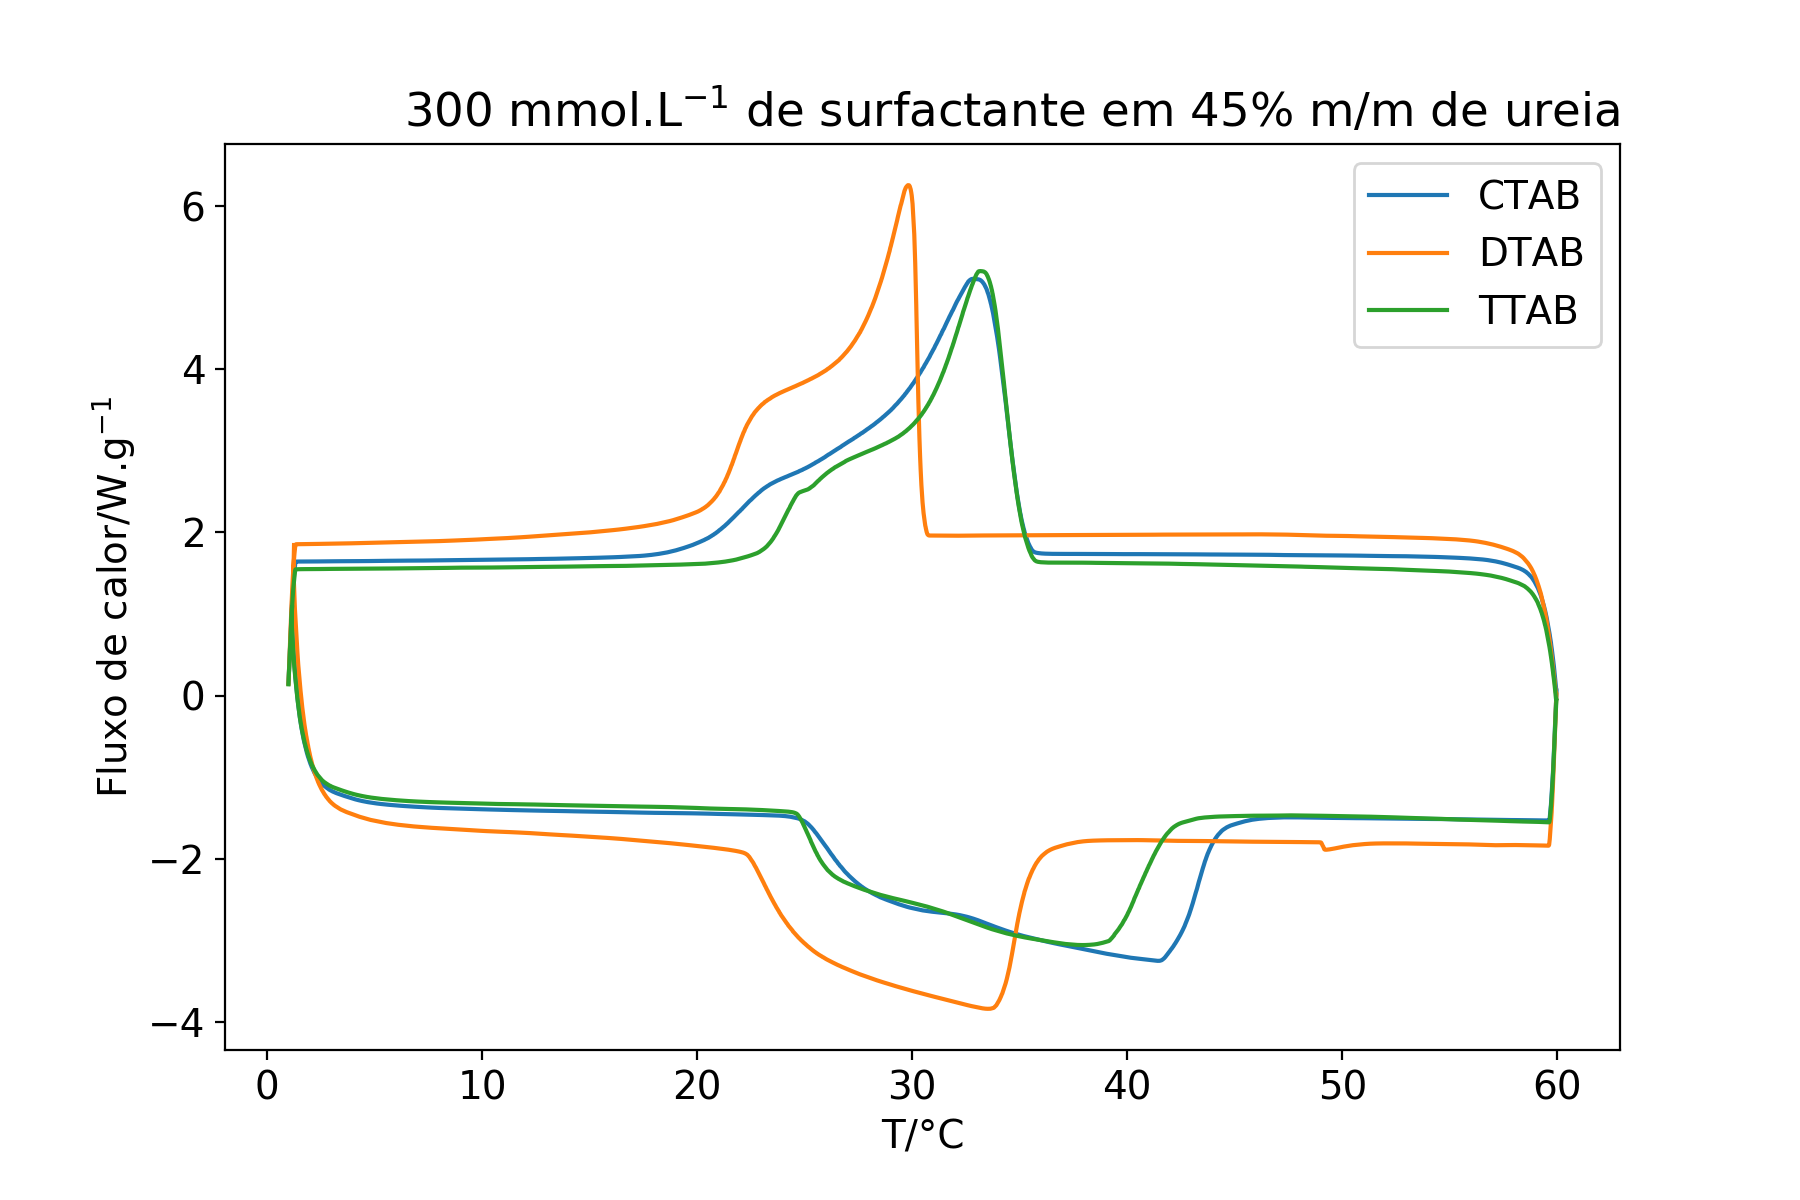
\includegraphics[width=0.60\textwidth]{./imagens/dsc/Surf_300mm_45p}
			\caption{Termogramas de soluções de (C|T|D)TAB 300 \mM{}, em 45\% de ureia}
			\label{fig:DSC_Surf_300mm_45p}
		\end{figure}
	
		\begin{figure}[H]
			\centering
			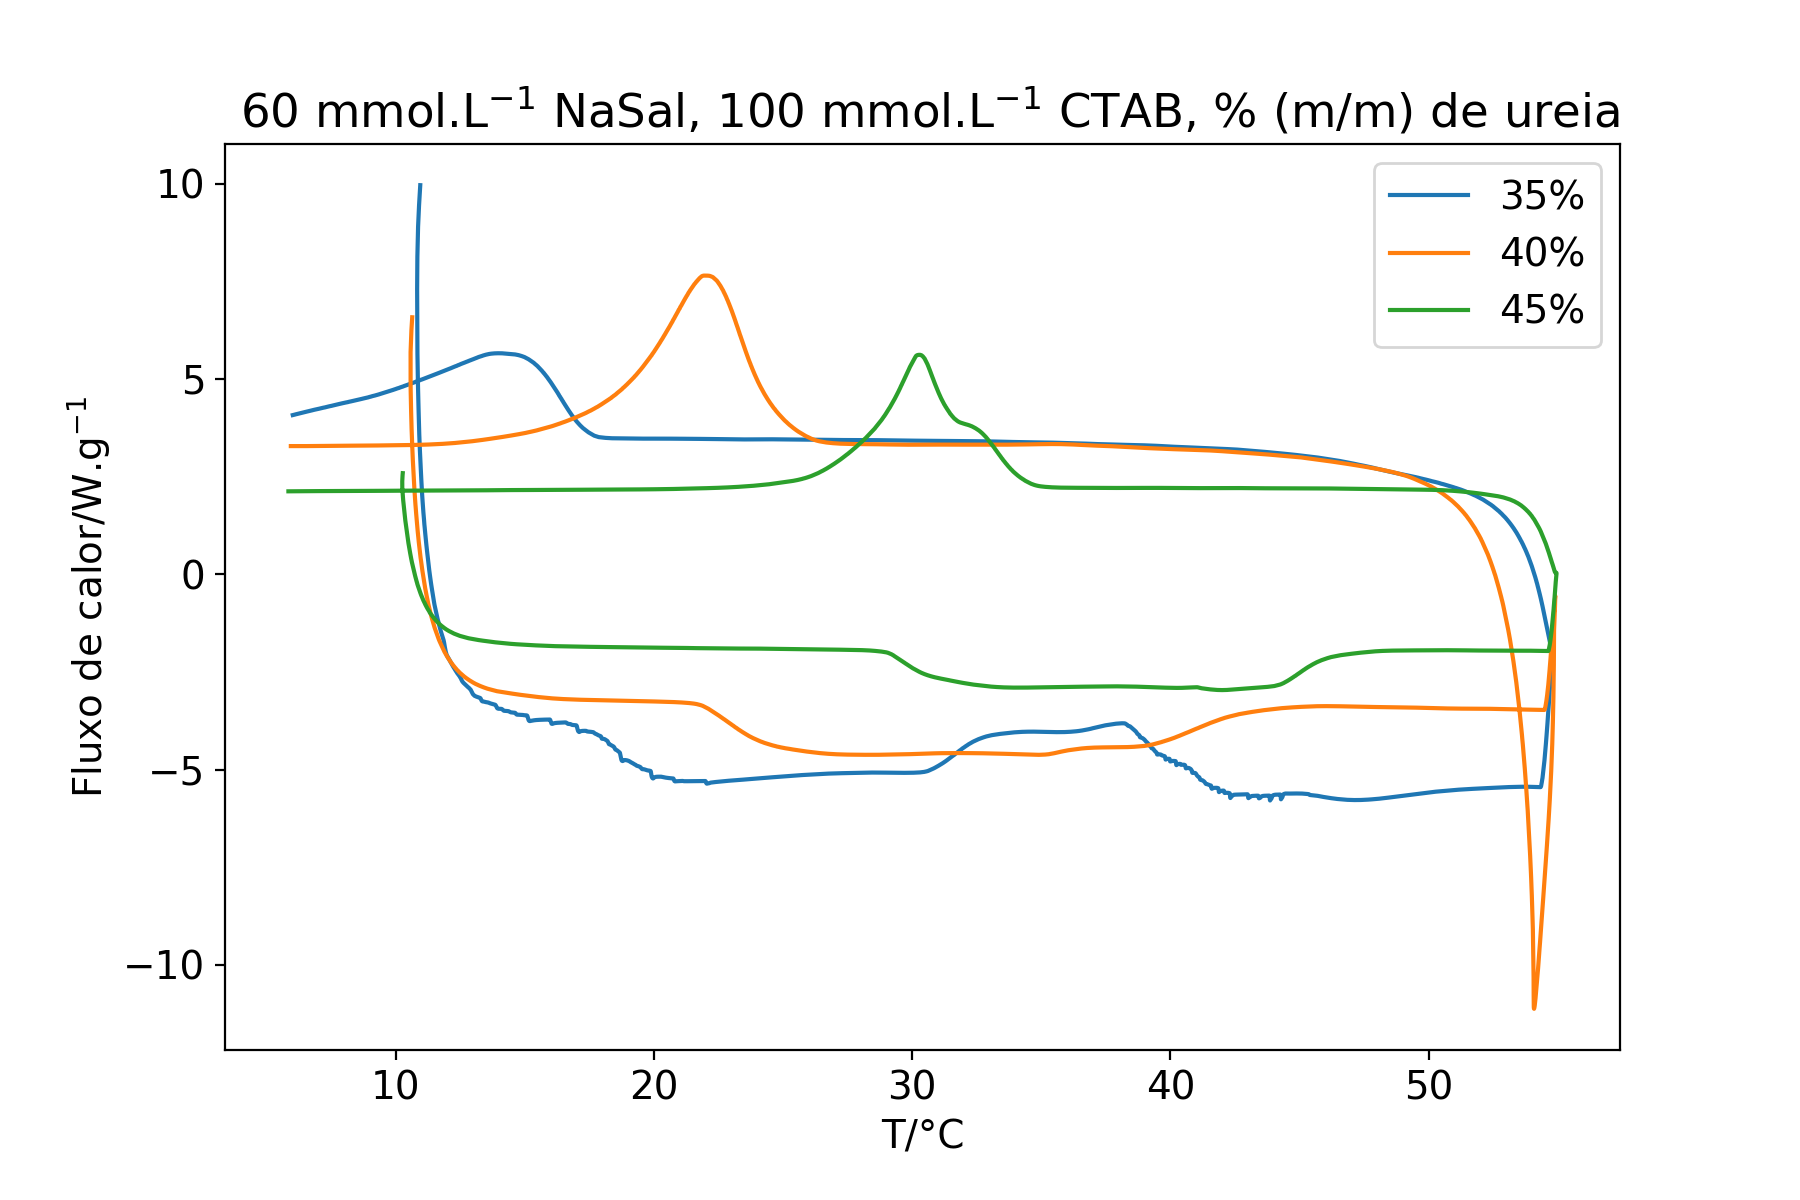
\includegraphics[width=0.60\textwidth]{./imagens/dsc/NaSal60}
			\caption{Termogramas de soluções de NaSal 60\mM{} e CTAB 100 \mM{}, em 35\%, 40\% e 45\% (m/m) de ureia}
			\label{fig:DSC_NaSal60}
		\end{figure}
	
		\begin{figure}[H]
			\centering
			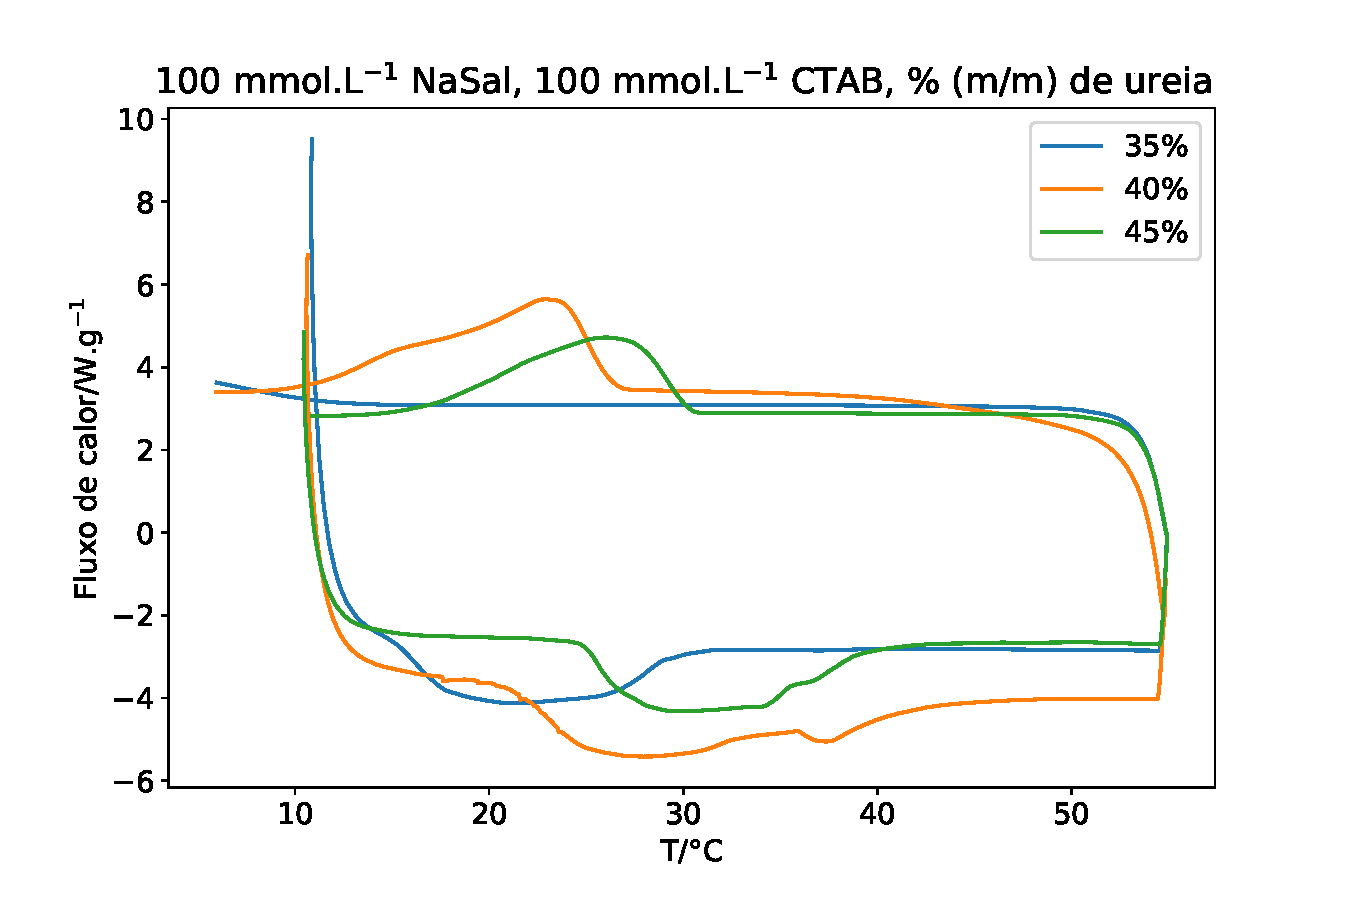
\includegraphics[width=0.60\textwidth]{./imagens/dsc/NaSal100}
			\caption{Termogramas de soluções de NaSal 100\mM{} e CTAB 100 \mM{}, em 35\%, 40\% e 45\% (m/m) de ureia}
			\label{fig:DSC_NaSal100}
		\end{figure}

		\begin{figure}[H]
			\centering
			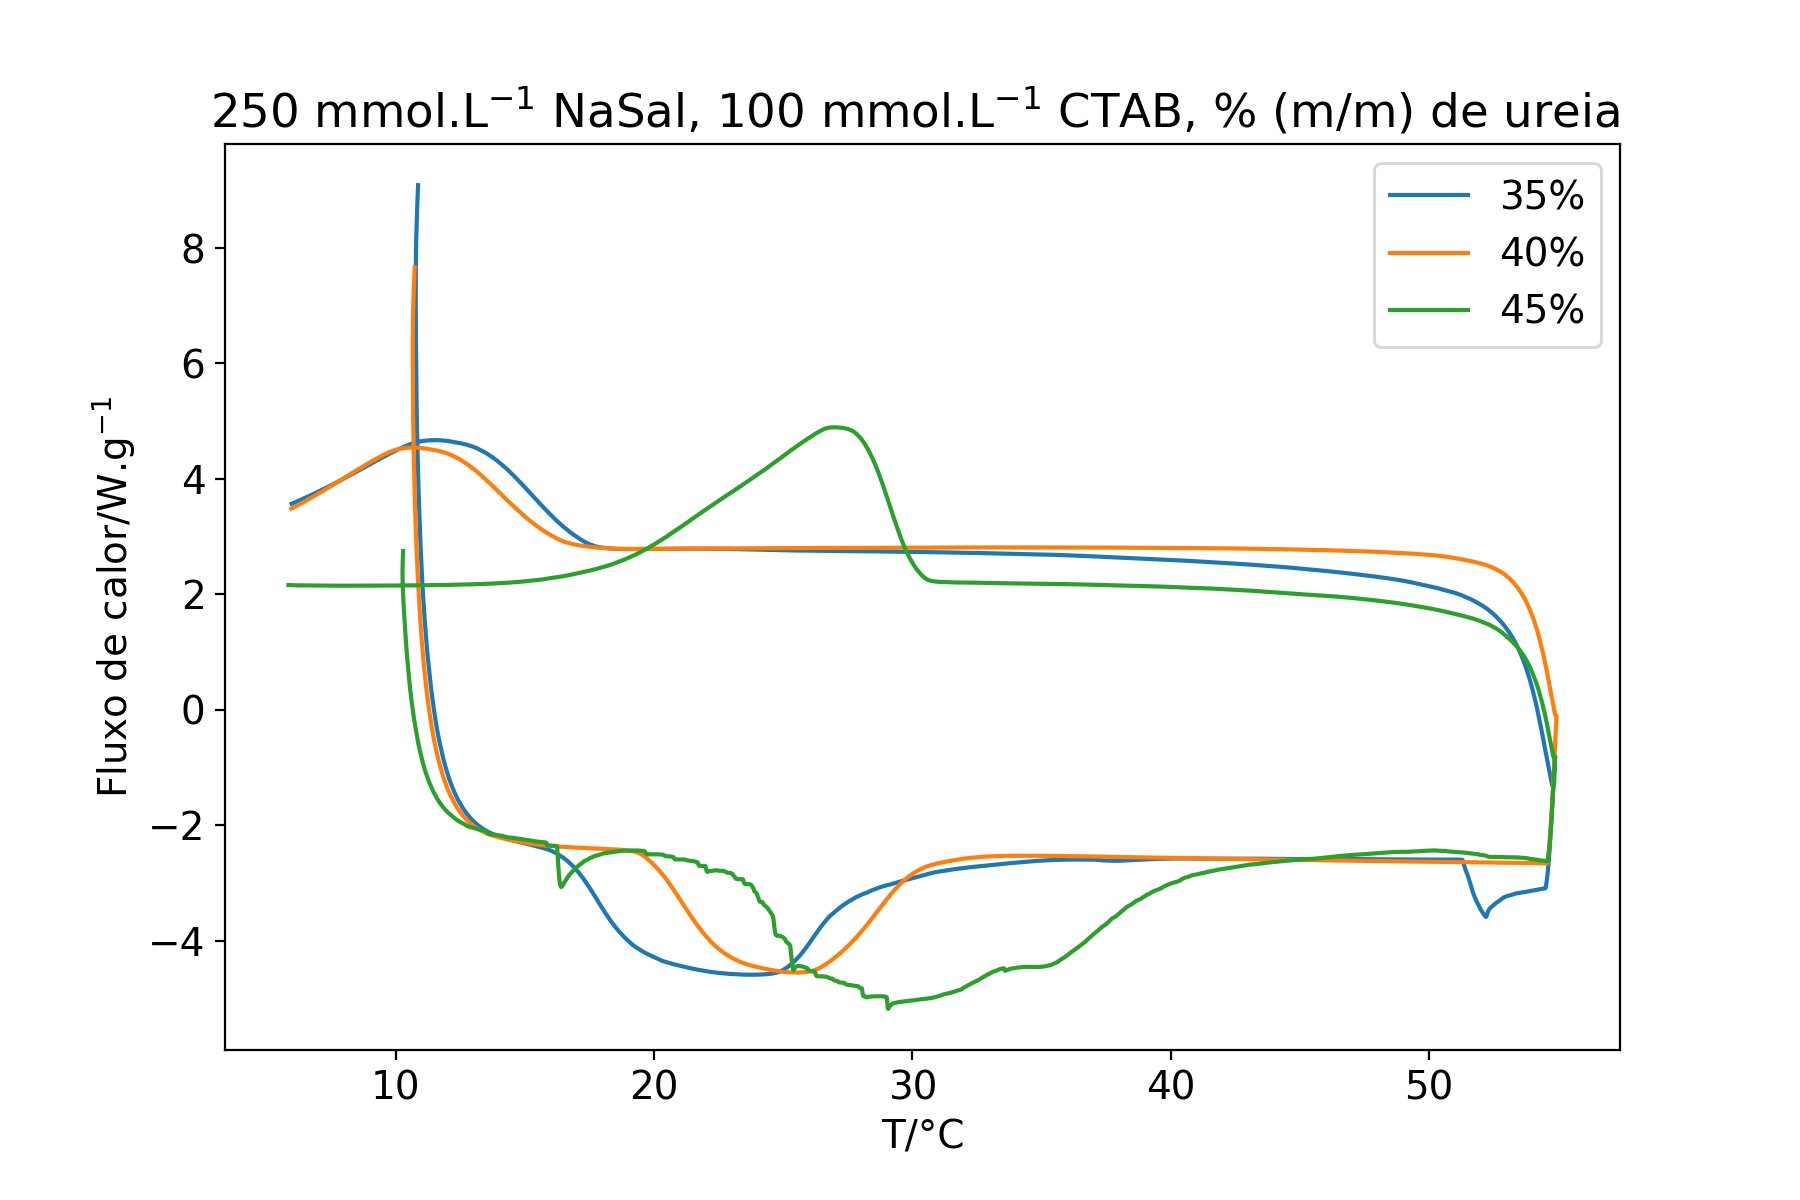
\includegraphics[width=0.60\textwidth]{./imagens/dsc/NaSal250}
			\caption{Termogramas de soluções de NaSal 250\mM{} e CTAB 100 \mM{}, em 35\%, 40\% e 45\% (m/m) de ureia}
			\label{fig:DSC_NaSal250}
		\end{figure}
	
		\begin{figure}[H]
			\centering
			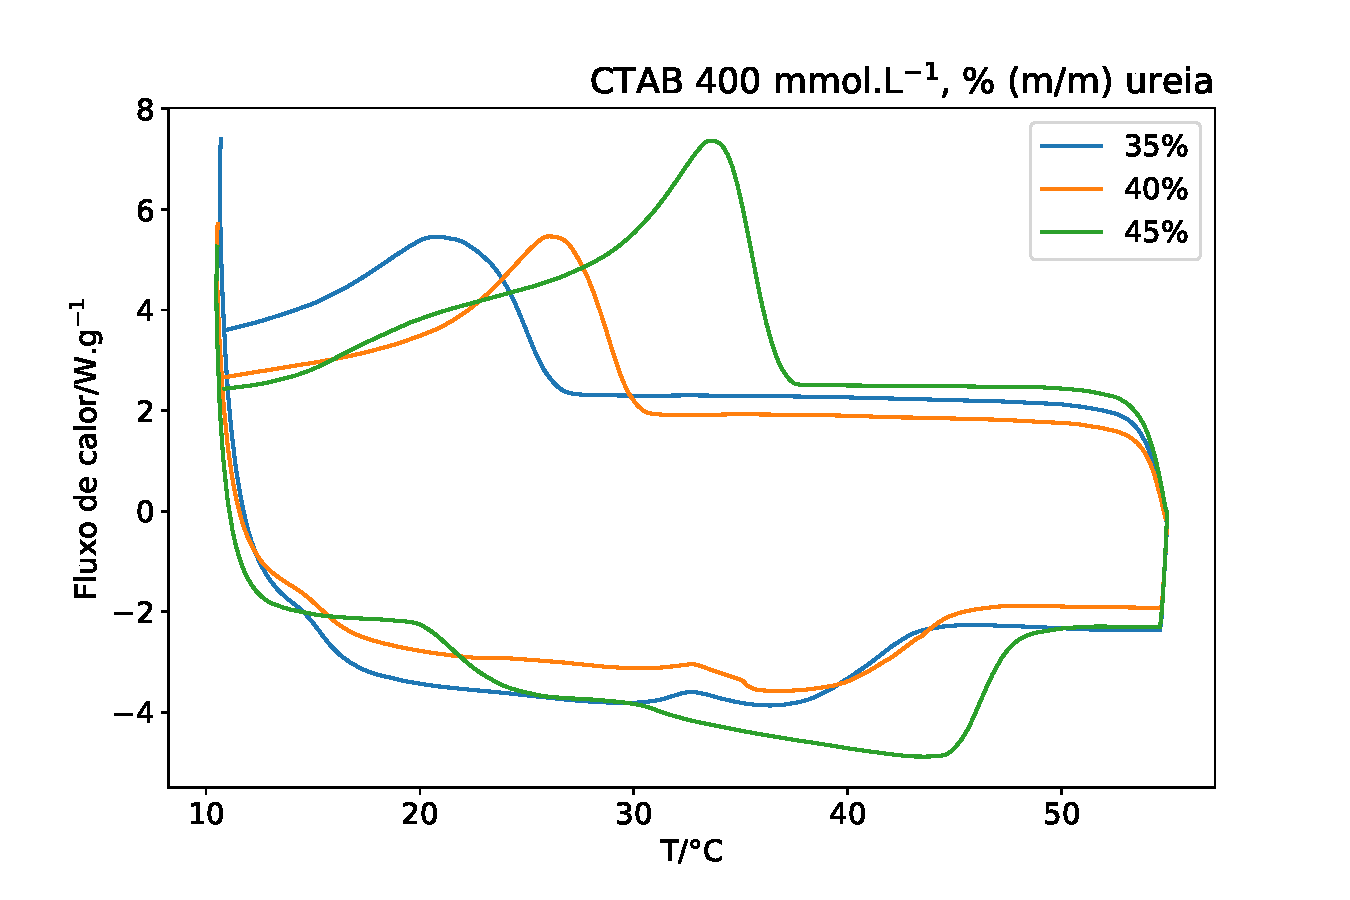
\includegraphics[width=0.60\textwidth]{./imagens/dsc/NaSal35}
			\caption{Termogramas de soluções de NaSal 60, 100 e 250\mM{} e CTAB 100 \mM{}, em 35\% (m/m) de ureia}
			\label{fig:DSC_NaSal_Ur35}
		\end{figure}
	
		\begin{figure}[H]
			\centering
			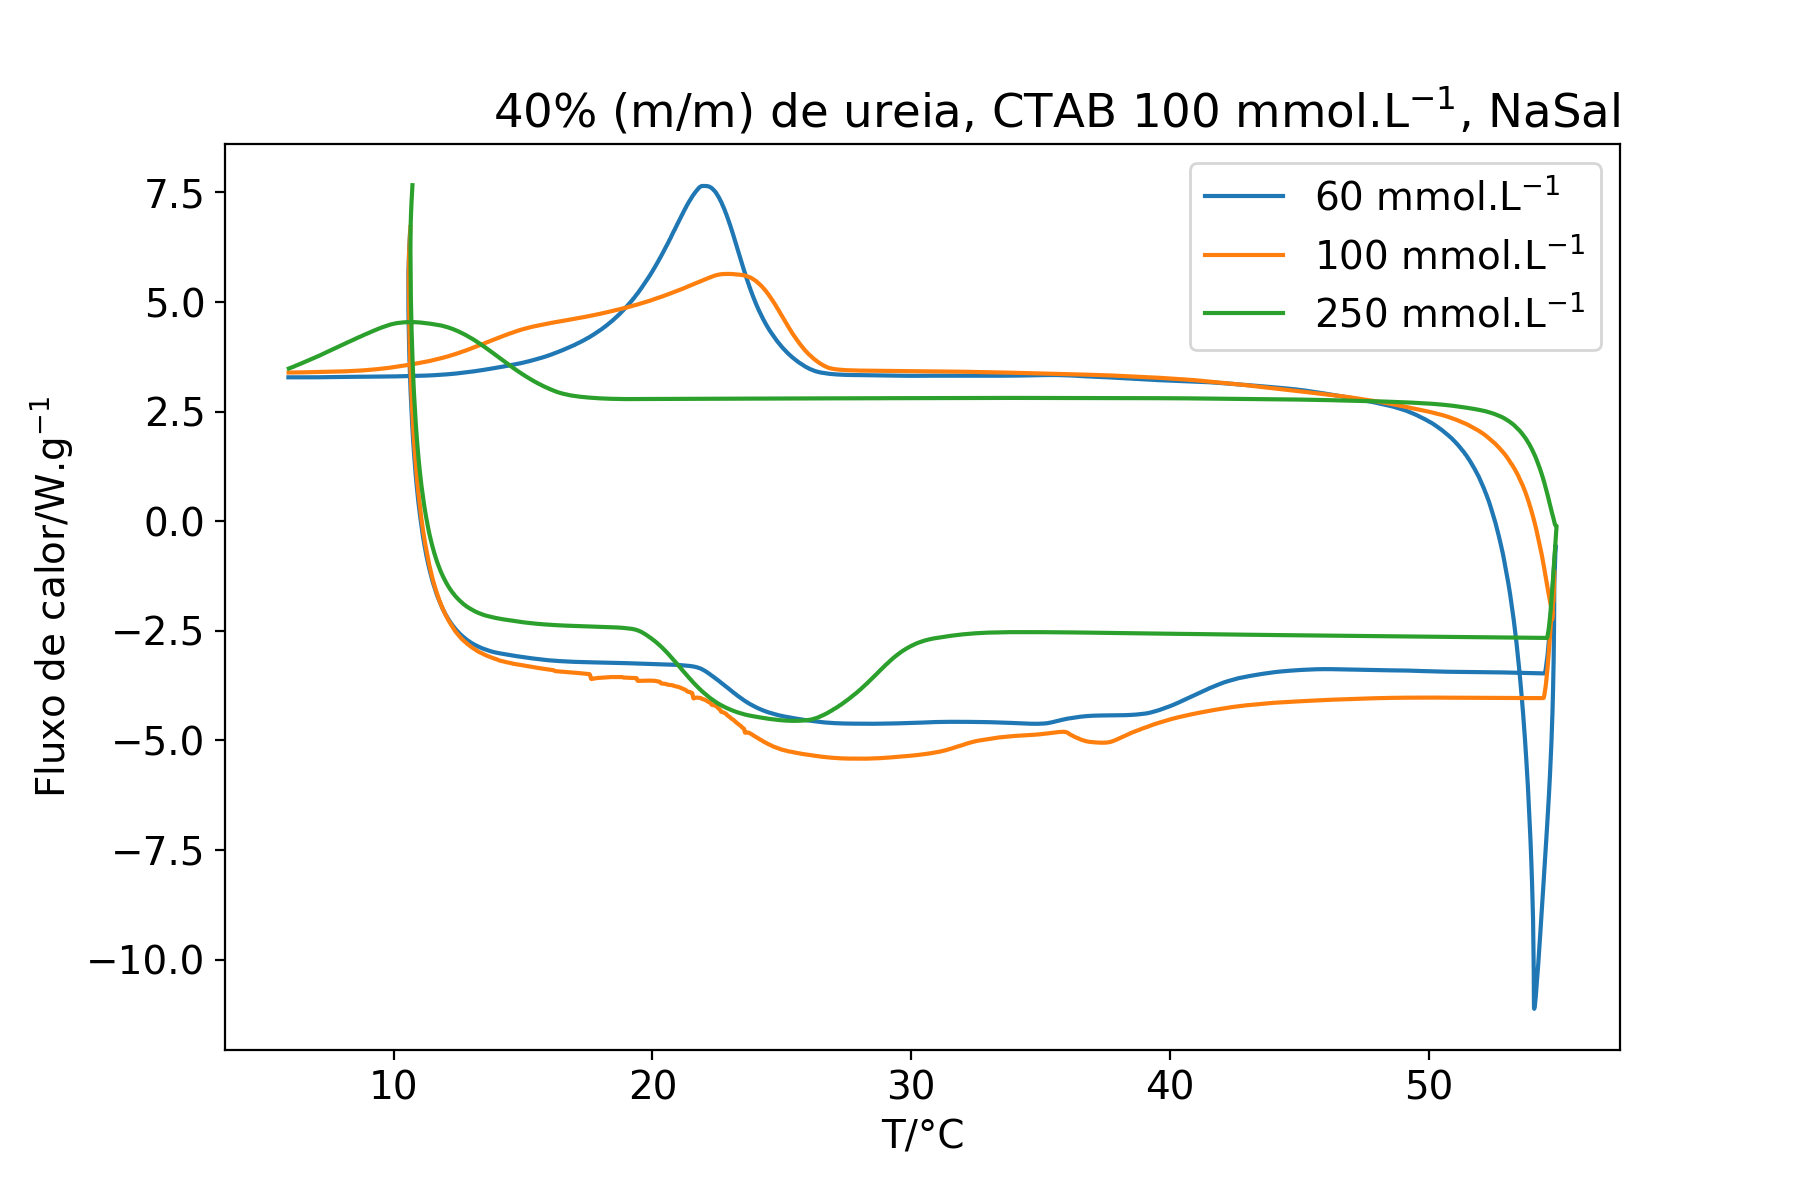
\includegraphics[width=0.60\textwidth]{./imagens/dsc/NaSal40}
			\caption{Termogramas de soluções de NaSal 60, 100 e 250\mM{} e CTAB 100 \mM{}, em 40\% (m/m) de ureia}
			\label{fig:DSC_NaSal_Ur40}
		\end{figure}

		\begin{figure}[H]
			\centering
			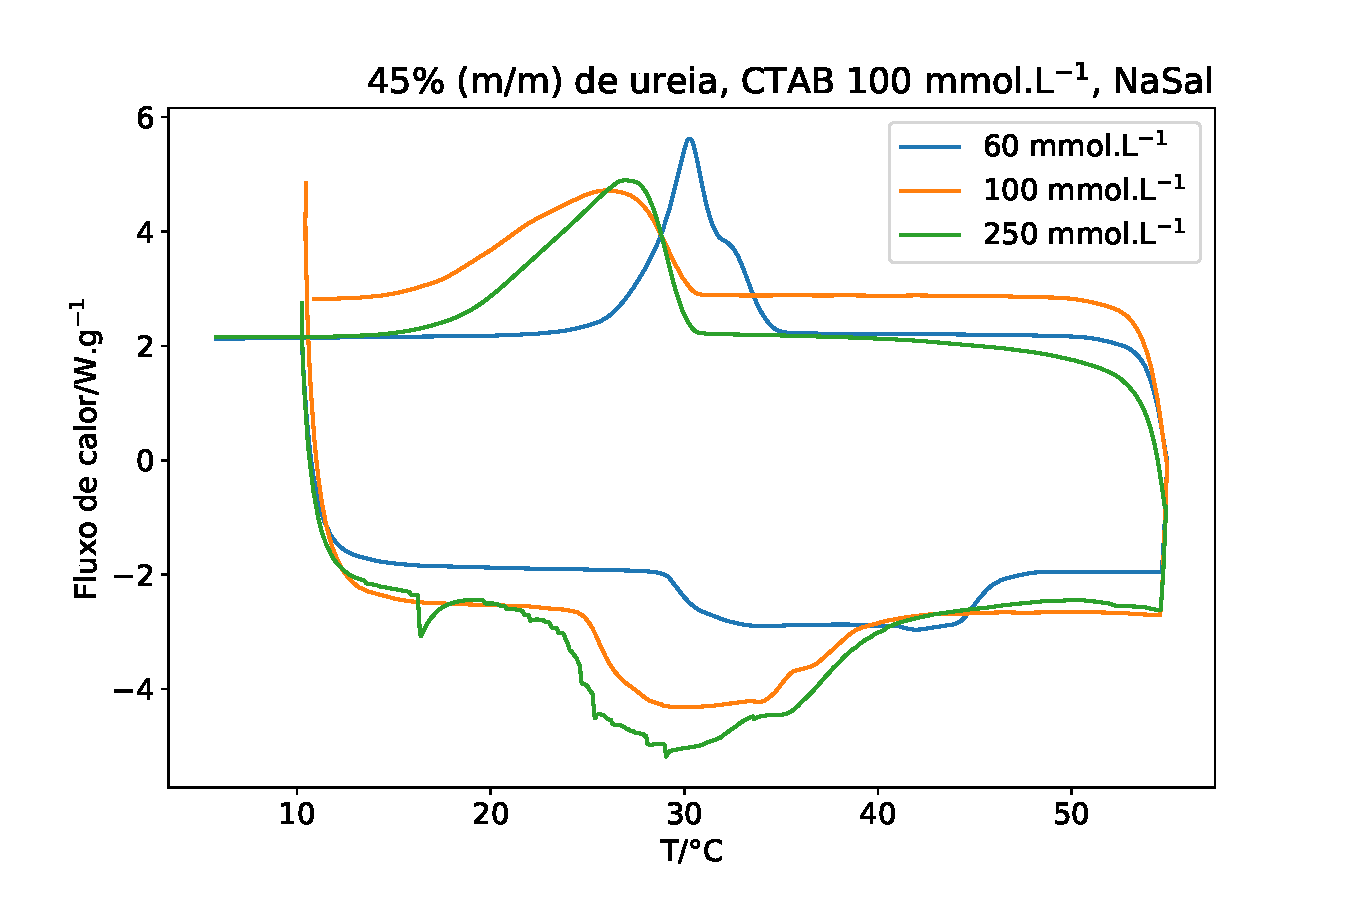
\includegraphics[width=0.60\textwidth]{./imagens/dsc/NaSal45}
			\caption{Termogramas de soluções de NaSal 60, 100 e 250\mM{} e CTAB 100 \mM{}, em 45\% (m/m) de ureia}
			\label{fig:DSC_NaSal_Ur45}
		\end{figure}

			
		% (Figs. \ref{fig:DSC_CTAB_UR38-45}, \ref{fig:DSC_CTAB_UR40-45}, \ref{fig:DSC_TTAB_UR_40-45}, \ref{fig:DSC_DTAB_UR_40-45}, \ref{fig:DSC_NaSal60}, \ref{fig:DSC_NaSal100}, \ref{fig:DSC_NaSal250})
		Qualitativamente, podemos observar que com o aumento de concentração de ureia, a temperatura de transição também aumenta. Além disso, vemos que CTAB e TTAB possuem temperaturas semelhantes de transição, maiores que DTAB (Figs. \ref{fig:DSC_Surf_100mm_45p}, \ref{fig:DSC_Surf_200mm_45p}, \ref{fig:DSC_Surf_300mm_45p}).
		
		% todo: será que dá pra fazer alguma análise estatística aqui? Ou plotar mais gráficos?
		
		As áreas de transição, e a largura dos picos são, também, proporcionais à concentração de surfactante utilizado. Quanto maior a concentração, maior 
		
		 A adição de NaSal causa uma diminuição na temperatura de transição, especialmente visível em 250\mM{} de NaSal. As tabelas \ref{tab:DSC_temp_areas} e \ref{tab:DSC_temp_areas_NaSal} mostram as temperaturas de transição no aquecimento e resfriamento, obtidas pelo valor do máximo do pico, as áreas de transição e as larguras a meia altura dos picos 

        \begin{table}[H]
            \IBGEtab%
            {\caption{Temperaturas de transição ($T$/°C), áreas de transição por mol de surfactante ($A$/$J.mol^{-1}$) e largura a meia altura dos picos de transição ($L$/°C) dos ciclos de aquecimento (\emph{aq}) e resfriamento (\emph{res}) para três surfactantes (Surf.), CTAB, TTAB, DTAB, cujas concentrações estão em \mM, em várias concentrações \% (m/m) de ureia}
            \label{tab:DSC_temp_areas}}%
            {\begin{tabular}{ccccccccc}
                \toprule
    			\% Ur. & Surf. & $C_{surf}$ &
    			$T_{aq}$ & $T_{res}$ & $A_{aq}$ & $A_{res}$ & $L_{aq}$ & $L_{res}$\\
    			\midrule
    			38 & CTAB & 100 & 30,5 & 19,3 & 2,67 & 2,68 & 5,6 &	3,0\\
    			39 & CTAB & 100 & 32,5 & 25,2 & 2,28 & 2,30 & 6,4 &	2,4\\
    			40 & CTAB & 100 & 33,3 & 25,1 & 4,73 & 4,41 & 5,6 &	3,0\\
    			41 & CTAB & 100 & 34,1 & 27,2 & 1,74 & 1,77 & 5,3 &	1,6\\
    			42 & CTAB & 100 & 37,5 & 29,6 & 2,71 & 2,75 & 6,0 &	1,9\\
    			43 & CTAB & 100 & 38,7 & 31,1 & 2,10 & 2,10 & 5,4 &	1,8\\
    			44 & CTAB & 100 & 40,2 & 34,6 & 1,86 & 1,85 & 4,9 &	1,6\\
    			45 & CTAB & 100 & 41,0 & 34,6 & 2,04 & 2,02 & 4,6 &	1,5\\
    			\midrule
    			40 & CTAB & 200 & 31,6 & 23,6 & 4,75 & 4,81 & 6,4 &	2,4\\
    			45 & CTAB & 200 & 41,6 & 34,9 & 1,72 & 1,92 & 10,3 & 3,5\\
    			40 & CTAB & 300 & 31,7 & 24,8 & 4,84 & 4,79 & 5,3 &	1,6\\
    			45 & CTAB & 300 & 41,4 & 32,8 & 2,40 & 2,44 & 15,4 & 5,8\\
    			35 & CTAB & 400 & 21,9 & 21,9 & 2,93 & 1,52 & 24,0 & 12,3\\
    			40 & CTAB & 400 & 36,4 & 26,5 & 2,99 & 1,78 & 23,3 & 7,4\\
    			45 & CTAB & 400 & 43,4 & 33,6 & 3,79 & 3,74 & 21,7 & 7,4\\
    			\midrule
    			40 & DTAB & 100 & 26,7 & 22,5 & 1,77 & 1,71 & 6,0 & 1,9\\
    			45 & DTAB & 100 & 33,0 & 30,1 & 1,39 & 1,48 & 2,5 & 1,1\\
    			40 & DTAB & 200 & 27,4 & 22,8 & 2,34 & 2,27 & 5,4 &	1,8\\
    			45 & DTAB & 200 & 33,4 & 30,0 & 1,83 & 1,88 & 6,3 &	2,8\\
    			40 & DTAB & 300 & 26,2 & 21,5 & 1,87 & 1,93 & 4,9 &	1,6\\
    			45 & DTAB & 300 & 33,5 & 29,8 & 2,04 & 2,13 & 10,6 & 3,7\\
    			\midrule
    			40 & TTAB & 100 & 31,9 & 26,4 & 4,94 & 5,04 & 4,6 &	1,5\\
    			45 & TTAB & 100 & 37,8 & 34,7 & 2,25 & 2,29 & 4,7 &	1,6\\
    			40 & TTAB & 200 & 31,9 & 25,3 & 3,94 & 4,00 & 10,3 & 3,5\\
    			45 & TTAB & 200 & 37,4 & 33,8 & 1,85 & 1,90 & 8,8 &	2,6\\
    			40 & TTAB & 300 & 29,8 & 26,5 & 4,81 & 4,61 & 15,4 & 5,8\\
    			45 & TTAB & 300 & 37,8 & 33,2 & 2,03 & 2,06 & 14,0 & 4,1\\
                \bottomrule
                \end{tabular}}%
            {}
        \end{table}
        
      \begin{table}[H]
          \IBGEtab%
          {\caption{Temperaturas de transição ($T$/°C), áreas de transição por mol de surfactante ($A$/$J.mol^{-1}$) e largura a meia altura dos picos de transição ($L$/°C) dos ciclos de aquecimento (\emph{aq}) e resfriamento (\emph{res}) para CTAB com NaSal, cujas concentrações estão em \mM, em três concentrações \% (m/m) de ureia}
          \label{tab:DSC_temp_areas_NaSal}}%
            {\begin{tabular}{cccccccccc}
                \toprule
                \% Ur. & Surf. & $C_{surf}$ & $C_{NaSal}$ &
                $T_{aq}$ & $T_{res}$ & $A_{aq}$ & $A_{res}$ & $L_{aq}$ & $L_{res}$\\
       			\midrule
       			35 & CTAB & 100 & 60 & 22,0 & 14,6 & 5,07 & 3,48 & - & -\\
       			40 & CTAB & 100 & 60 & 27,6 & 22,0 & 6,67 & 6,18 & - & -\\
       			45 & CTAB & 100 & 60 & 42,0 & 23,5 & 5,66 & 4,06 & 15,0 & 3,0\\
       			35 & CTAB & 100 & 100 & 20,7 & - & 5,00 & - & 10,9 & -\\
       			40 & CTAB & 100 & 100 & 27,1 & 22,9 & 7,03 & 5,82 & 15,3 &	9,1\\
       			45 & CTAB & 100 & 100 & 29,9 & 26,0 & 5,51 & 4,87 & 11,0 &	8,5\\
       			35 & CTAB & 100 & 250 & 22,8 & 12,7 & 6,05 & 2,98 & 8,5 &	8,7\\
       			40 & CTAB & 100 & 250 & 23,3 & 11,8 & 4,55 & 2,60 & 7,1 &	7,5\\
       			45 & CTAB & 100 & 250 & 29,1 & 27,0 & 9,99 & 5,93 & 12,3 &	6,9\\
       			\bottomrule
            \end{tabular}}%
                {}
            \end{table}

		
	\section{SAXS}
	\section{DLS}
	\section{Reologia do sólido}
	\section{Entalpia de interação de ureia com surfactante}